% \chapter{METHODOLOGY}

\begin{sloppypar}
	
	\section{Introduction}
	In this chapter, we explore our data, perform data preparations, and feature engineering on the dataset, then we build, compare, and evaluate three models: neural network, linear, and ridge regression.


	\section{Exploratory Data Analysis}
	Exploratory data analysis refers to the critical process of performing initial investigations on data to discover patterns, spot anomalies, test hypotheses, and check assumptions with the help of summary statistics and graphical representations \citep{Patil}. Visualizations not shown in this section are allocated in the appendix. \newline
	Figure \ref{fig:t2} shows skewed data of the target feature and \ref{fig:lnp1} shows the transformation of the target feature using a natural log, which is deemed to have a normal distribution.
	
	\begin{figure}[h!]
	\centering	
	\begin{subfigure}{0.49\textwidth}
		\centering
		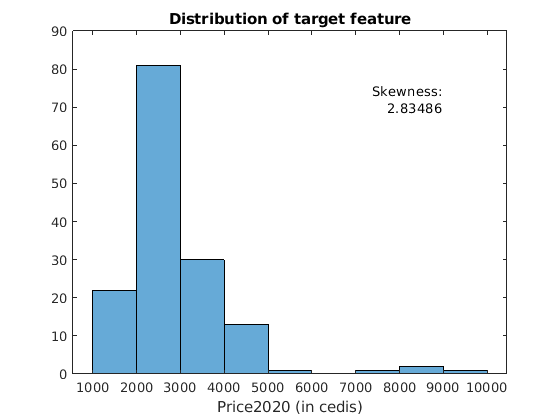
\includegraphics[width=\textwidth]{target2}
		\caption{Distribution of price2020}
		\label{fig:t2}
	\end{subfigure}
	\hfill
	\begin{subfigure}{0.49\textwidth}
		\centering
		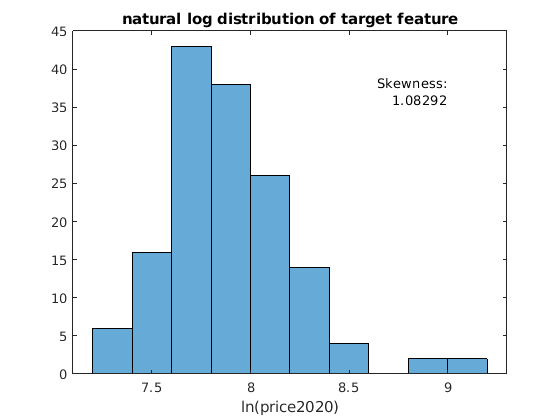
\includegraphics[width=\textwidth]{lnprice1}
		\caption{Distribution of ln(price2020)}
		\label{fig:lnp1}
	\end{subfigure}
	\caption{Histograms of target feature 1}	
	\label{fig:dist}
	\end{figure}

	
	\section{Data Preparation}
	Data preparation is the act of manipulating raw data (which may come from disparate data sources) into a form that can readily and accurately be analyzed \citep{Davidf}. In light of that, we first deal with missing data and remove inputs that behave like outliers. Next, we select important features and feature engineer the categorical features.

	\subsection{Missing Data}
	Most \ac{ml} algorithms cannot work with missing features \citep{Douglass2020}. Missing data are unobserved values that would be meaningful for analysis if observed. In other words, a missing value hides a meaningful value \citep{little1988}.
	
	\begin{table}[h!]
		\centering
		\caption{Missing Data in hostels dataset}
		\label{table:3}
		\begin{tabular}{|c|cccc|}
			\hline
			\textbf{Feature} & grade & rank & price2018 & price2019 \\ \hline
			\textbf{\%Missing} & 3\% & 3\% & 89\% & 64\% \\
			\textbf{numMissing} & 5 & 5 & 135 & 97 \\ \hline
			\textbf{numTotal} & \multicolumn{4}{|c|}{242} \\ \hline
		\end{tabular}
	\end{table}
	
	\hspace*{-0.6cm}The two types of missingness observed in our dataset are \ac{mar} and \ac{mcar}. The grade is of type \ac{mcar} since respondents chose to skip answering; hence they were fixed using the imputation method. Rank is of type \ac{mar} considering its value depends on the grade. price2018 and price2019 are of type \ac{mcar} because, in most cases, respondents were not present in their hostels during those academic years and thus discarded completely.
	
	\subsection{Outliers}
	By default, an outlier is a value that is more than three scaled \ac{mad} away from the dataset \citep{Mathworks}. Outliers can easily affect the performance of the model\citep{Parashar2021}. Hence, we use $ 99\% $ of our dataset to reduce their effect on the data (and models).
	
	\subsection{Feature Selection} 
	Feature selection is a subfield within \ac{ml} aimed at creating accurate models by excluding irrelevant features and including only relevant features \citep{Jaiantilal2013}. Features are selected based on their scores in various statistical tests (e.g., Pearson's correlation) for their correlation with the outcome variable.
	
	\subsection{Feature Engineering}
	Every \ac{ml} model is based on some mathematical concept, so we encode every categorical value into a numerical value. Features without inherent order, such as study\_room were one-hot-encoded, and features with inherent order, such as rank, were label encoded.
	Also, beds and post\_code features were deemed categorical since they contain 4 and 21 distinct responses, respectively, with no inherent order. Therefore, we one-hot-encoded the two features.
	
	\subsection{Data Splitting}
	Data splitting is the process of partitioning our available data into a train set (for training all models) and a test set (to evaluate the models). Using the cvpartition object together with the Mersenne Twister random number generator (i.e., rng (1)) in Matlab (R2021a), the cleaned dataset will be randomly partitioned, with 65\% as a training set and 35\% as a test set.
	
	
	\section{Model Selection}
	\subsection{Criteria to Measure Performance}
	The test set were evaluated using: \ac{mae}, \ac{rmse} and Coefficient of Determination ($ R^2 $)
	
	\subsubsection{Mean Absolute Error (MAE)}
	\begin{equation} \label{eqn:mae}
	MAE = \frac{1}{n}\sum_{i=1}^{n} |e_i| = \frac{1}{n}\sum_{i=1}^{n} |y_i - \hat{y}_i|
	\end{equation}
		
	\subsubsection{Root Mean Squared Error (RMSE)}
	\begin{equation} \label{eqn:rmse}
		RMSE = \sqrt{ \frac{1}{n} SSE } = \sqrt{ \frac{1}{n} \sum_{i=1}^{n} (y_i - \hat{y}_i)^2 } 
	\end{equation}
	
	\subsubsection{Coefficient of Determination ($R^2$)}
	\[SST = \sum_{i=1}^{n} (y_i - \bar{y})^2 \ \ \ \ \ \ \ SSE =  \sum_{i=1}^{n} (y_i - \hat{y})^2 \]
	\begin{equation} \label{eqn:r2}
	R^2 = 1 - \frac{SSE}{SST}
	\end{equation}
	
	\subsection{Predictive Modeling}
	\subsubsection{Linear Regression}
	Linear regression \citep{Chatterjee2013} is a linear approach to modeling the relationship between a response and one or more explanatory variables. Given a dataset $ \{x_{1i}, x_{2i}, ..., x_{pi}, y_i\} $ of $ n $ sets of observations, it is assumed that these observations satisfy a linear relationship,
	\begin{equation} \label{eqn:mlr}
	y_i = \beta_o + \beta_1 x_{1i} + \beta_2 x_{2i} + \cdots + \beta_p x_{pi} + \epsilon_i = X \beta + \epsilon
	\end{equation}
	A primary goal of regression analysis is to estimate the unknown parameters $ \beta$. The standard approach is least squares regression, where the estimates chosen to minimize are,
	\begin{equation} \label{eqn:ols}
	\norm{y - X\beta}_2^2 = \sum_{i=1}^{n} [ y_i - (\beta_o + \beta_1 x_{1i} + \cdots + \beta_p x_{pi}) ]^2
	\end{equation}
	
	\hspace*{-0.6cm}The normal equation which determines the minimizer of \ref{eqn:ols} is,
	\begin{equation}
	\hat{\beta} = (X^{T}X)^{-1}X^{T}y
	\end{equation}
	
	\subsubsection{Ridge Regression}
	\ac{rr} \citep{Shewhart2015} is a method of estimating the coefficients of \ac{mlr} models in scenarios where independent variables are highly correlated. \newline
	The theory was first introduced by Hoerl and Kennard in 1970 \citep{hoerl1970ridge}. However, \ac{rr} is a special case of Tikhonov regularization \citep{tikhonov1966stability}, in which all parameters are equally regularized. The \ac{prss} is,
		\begin{equation} \label{eqn:prss}
		\norm{y - X\beta}_2^2 + \lambda \norm{\beta}_2^2
		\end{equation}
		\ac{rr} estimate coefficients in \ref{eqn:prss} using
		\begin{equation}
		\hat{\beta}_{ridge} = (X^{T} X + \lambda I)^{-1} X^{T} y
		\end{equation}
		Where $ \lambda $ is the shrinkage parameter and $ I $, an identity matrix.
	
	\subsubsection{Neural Network}
	\ac{nn} is an interconnected group of nodes inspired by a simplification of neurons in the brain. The network learns by adjusting weights to reduce the prediction error\citep{han2011data}. Initially, all weights and biases are randomly allocated. The algorithm then runs iteratively, and each iteration comprises two steps: forward feeding and backpropagation \citep{Phan2019}.

		\begin{itemize}%[leftmargin=*]
			\item In the forward feeding phase, the output for the computation unit, $ a_i^{k+1} $ is the result of applying a transfer function, $ \sigma $ to the summation of all signals from each connection, $ a_i^k $ times the value of the connection weight, $ W_{ji} $ between node $ a_i^{k+1} $ and connection $ a_i^{k} $ \citep{coakley2000artificial}. The prediction of the output layer is then compared to the observed outcome to derive the learning rate and errors \citep{Phan2019}.
			\begin{eqnarray}
			z_j = \sum_j (W_{ji}^k a_i^k) \\
			a_i^{k+1} = \sigma (z_j)
			\end{eqnarray}
			\begin{equation*}
			where \ \ \ \sigma = ReLU(x) = max(0,x)
			\end{equation*}
			
			where $a$ is the activation of unit $ i $ in layer $ k $, $W_j$ is the weight of unit $ i $ in layer $ k $  and $\sigma$ is the transfer function, \ac{relu}.
			
			\item In backpropagation, given the learning rate and errors, the network recalculates the weights and bias in hidden layers and makes appropriate changes to reduce prediction errors \citep{Phan2019}.
		\end{itemize}
	
\end{sloppypar}